% ==================================================
% 4.4 全身協同操作與預測時域比較
% ==================================================
\section{全身協同操作與預測時域比較}
\label{sec:wholebody_horizon_comparison}

全身控制需在底盤移動的同時維持末端追蹤，
並使手臂設定點的累積與關節響應符合物件操作需求。
本節以獨立抽屜場景分析底盤與手臂的運動分工，
再比較單步與五步控制的追蹤、命令變化及計算成本，
最後以完整開關抽屜與返回任務，比較移動中操作與停駐後操作的時間。
各組資料沿用取得時的控制與接觸設定；
本節操作目標由場景幾何建立，住宅場景的視覺導引與任務整合於第 4.5 節說明。

% ==================================================
% 4.4.1 底盤與末端協同追蹤表現
% ==================================================
\subsection{底盤與末端協同追蹤表現}
\label{subsec:base_tcp_coordinated_tracking}

抽屜場景使用具有單一滑動自由度的被動機構，
把手橫桿直徑為 $26$ mm，目標開度為 $200$ mm。
控制週期為 $0.05$ s，物理步長為 $0.01$ s，
手臂仍以設定點變化率作為輸入。
任務依序執行接近、夾持、拉開、開啟保持、推回、關閉保持與退出，
再收臂並返回起點。
開啟與關閉分別要求在 $195$--$205$ mm 與 $0$--$5$ mm 的範圍連續保持至少 $2$ s；
夾持建立則要求雙指接觸力皆達 $0.5$ N 並連續維持至少 $2$ s。
底盤配合滑軌方向移動，手臂同步調整構型以追蹤把手位姿。

為呈現兩者的幾何分工，令
$f(b,q_a)$ 表示由底盤位姿與手臂構型計算的 TCP 世界位置，
$b_0,q_{a,0}$ 為拉開開始時的構型，
$a_d$ 為滑軌開啟方向的單位向量。
依序代入底盤與手臂構型，定義軸向位移分量：
\begin{equation}
    \begin{aligned}
        \Delta\ell_B(t)
        &=a_d^\top\!\left[f(b(t),q_{a,0})-f(b_0,q_{a,0})\right],\\
        \Delta\ell_A(t)
        &=a_d^\top\!\left[f(b(t),q_a(t))-f(b(t),q_{a,0})\right],\\
        \Delta\ell_E(t)&=\Delta\ell_B(t)+\Delta\ell_A(t).
    \end{aligned}
    \label{eq:ch4_coordinated_displacement_decomposition}
\end{equation}
底盤分量包含平移與偏航對 TCP 的共同作用，
手臂分量則在當時底盤位姿下計算。
此分解為構型變化的幾何描述，其數值依上述代入順序定義。

以時域比較中配對案例一的五步控制紀錄為例，
\cref{fig:ch4_wholebody_drawer_coordination}(a)顯示拉開至推回期間的位移。
開始開啟保持時，TCP 沿滑軌方向累積移動約 $195.2$ mm，
其中底盤與手臂幾何分量分別約為 $139.6$ 與 $55.7$ mm。
推回時，兩者共同減少末端的軸向位移，
使 TCP 隨把手返回關閉位置。
這項結果呈現底盤對操作位移的實際參與，
手臂同時承接末端追蹤所需的剩餘構型變化。

\begin{figure}[htbp]
    \centering
    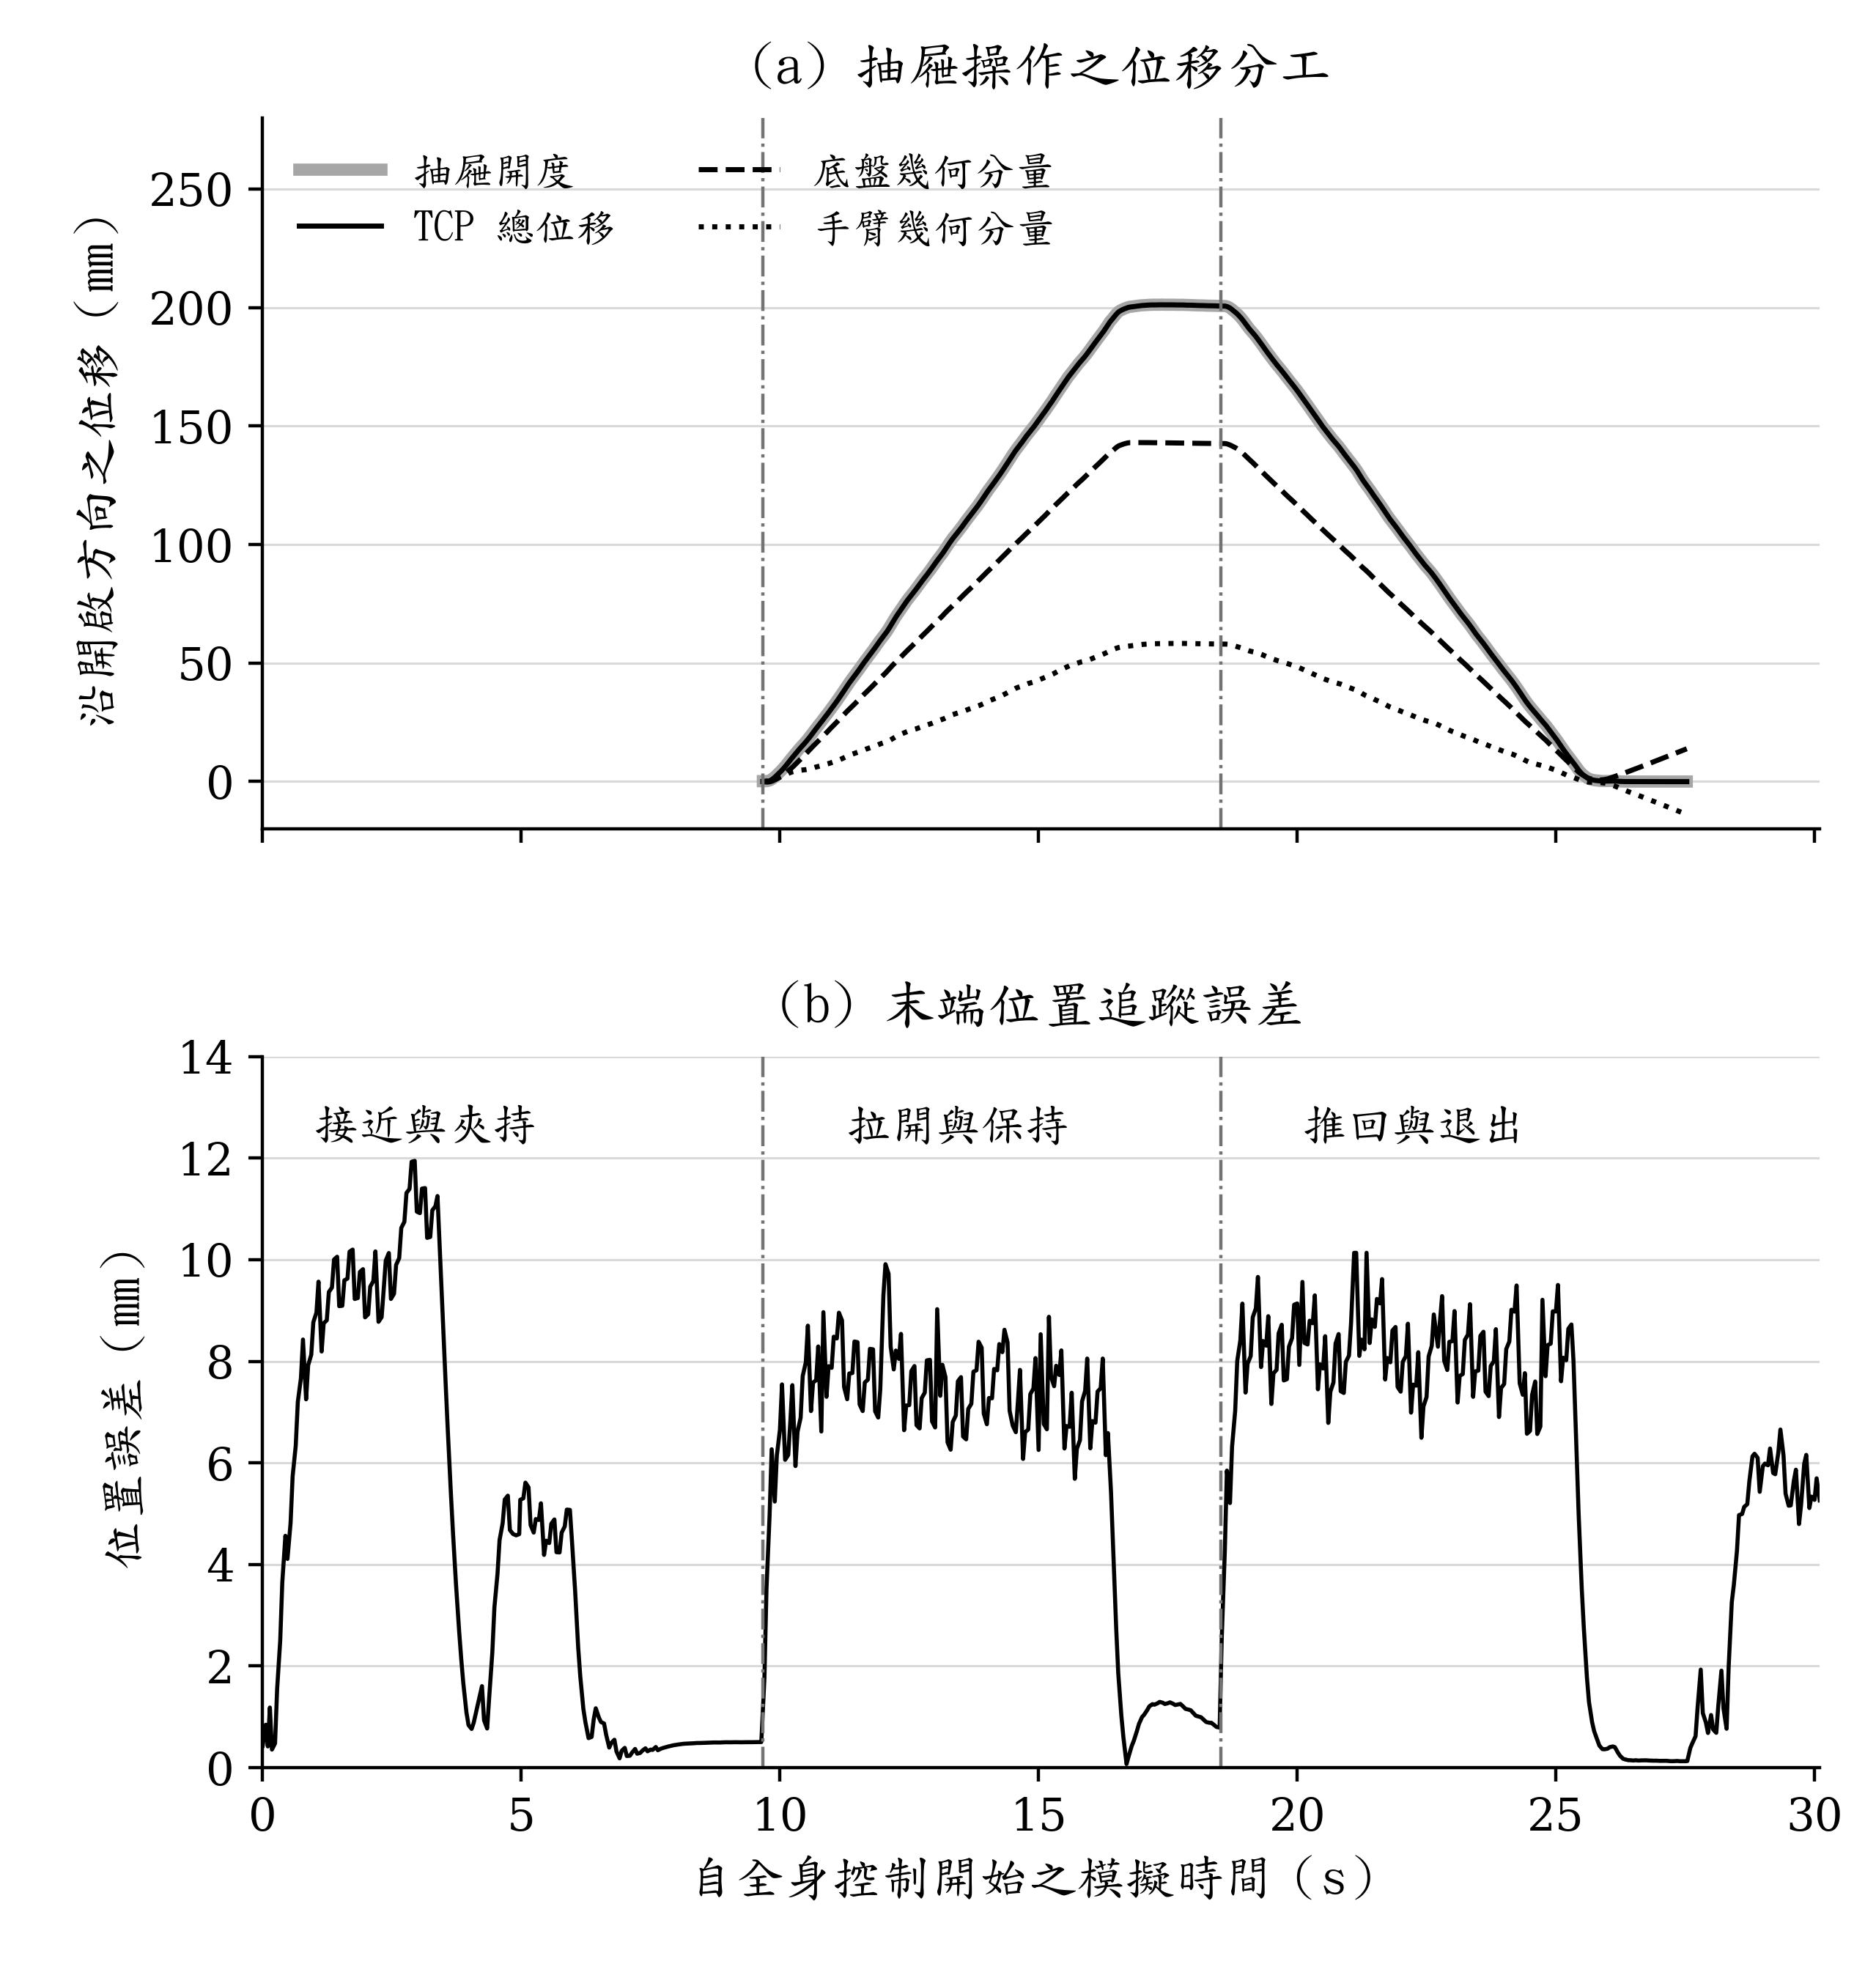
\includegraphics[width=0.98\textwidth]{figsrc/ch04/wholebody_drawer_coordination.png}
    \caption{配對案例一之五步全身控制結果：
    (a) 抽屜開度、TCP 軸向總位移與底盤及手臂幾何分量，位移以拉開起點為基準；
    (b) 全身控制區間之末端位置追蹤誤差。
    點畫直線分別標示拉開與推回開始時刻。}
    \label{fig:ch4_wholebody_drawer_coordination}
\end{figure}

\cref{fig:ch4_wholebody_drawer_coordination}(b)呈現同一案例的末端位置誤差。
接近、拉開與推回期間的誤差高於定點保持階段，
因此整段追蹤統計需配合任務階段解讀。
三個五步控制案例的位置誤差第 $95$ 百分位數為 $7.27$--$9.75$ mm，
姿態誤差第 $95$ 百分位數為 $0.207$--$0.300^\circ$。
實際關節位置與設定點至有效限位的最小餘量，
分別約為 $0.785$--$0.795$ rad 與 $0.783$--$0.793$ rad，
顯示此組運動仍保留關節範圍。
以下進一步比較相同任務下，預測步數改變所伴隨的追蹤與命令差異。

% ==================================================
% 4.4.2 單步與多步控制之比較
% ==================================================
\subsection{單步與多步控制之比較}
\label{subsec:single_multistep_control_comparison}

時域比較使用同一設定點增廣控制模型，
分別設定 $N=1$ 與 $N=5$，對應 $50$ 與 $250$ ms 的預測長度。
兩組共用任務流程、追蹤權重、命令限制與執行補償設定，
並以三組配對案例比較。
預測期間重複使用當輪取得的末端目標與協同參考，
未提供未來操作目標序列。
主要設定如\cref{tab:ch4_horizon_control_settings}所示。

\begin{table}[htbp]
    \centering
    \caption{單步與五步控制之比較設定}
    \label{tab:ch4_horizon_control_settings}
    \begingroup
    \small
    \renewcommand{\arraystretch}{1.2}
    \begin{tabular}{p{0.38\textwidth} c c}
        \hline
        項目 & 單步控制 & 五步控制 \\
        \hline
        預測步數 $N$ & $1$ & $5$ \\
        控制步長 & $0.05$ s & $0.05$ s \\
        預測時間長度 & $0.05$ s & $0.25$ s \\
        控制序列變數數量 $9N$ & $9$ & $45$ \\
        終端任務追蹤倍率 & $5$ & $5$ \\
        輸入與協同成本累加步數 & $1$ & $5$ \\
        時域內目標 & 當輪目標固定 & 當輪目標固定 \\
        配對案例數 & $3$ & $3$ \\
        \hline
    \end{tabular}
    \endgroup
\end{table}

終端倍率相同仍會隨預測步數改變成本結構。
令 $\ell_{T,i}$ 為第 $i$ 步受終端倍率作用的任務追蹤成本，
$\ell_{O,i}$ 為同一步對應的其餘輸入、命令變化與協同成本，
則兩組累加形式為
\begin{equation}
    \begin{aligned}
        J_{N=1}&=5\ell_{T,1}+\ell_{O,1},\\
        J_{N=5}&=\sum_{i=1}^{4}\ell_{T,i}
                   +5\ell_{T,5}+\sum_{i=1}^{5}\ell_{O,i}.
    \end{aligned}
    \label{eq:ch4_horizon_cost_accumulation}
\end{equation}
單步的唯一追蹤項即為放大的終端項，
五步則同時包含前四步追蹤與五份其餘成本。
因此，本組結果反映預測長度、終端項位置及成本累加比例共同形成的控制表現。

追蹤與命令統計的評估區間由首輪全身求解開始，
至退出完成且求解節點停止為止，
不包含進場導航、前段展臂、後續收臂與返回。
命令增量採相鄰求解輪送出的六軸手臂命令，
每次取各軸絕對差的最大值，再統計第 $95$ 百分位數。
其單位仍為 rad/s，表示設定點變化率的差異。
命令反轉則逐軸計算同一階段內，
相鄰兩輪絕對值皆大於 $0.05$ rad/s 且符號相反的次數，
再以整段控制時間換算反轉率。

六個案例皆完成任務並通過既定操作判準。
\cref{tab:ch4_horizon_control_results}列出三個案例各自統計值的範圍，
\cref{fig:ch4_horizon_tracking_comparison}則保留同一案例的配對關係。
五步控制的位置誤差第 $95$ 百分位數為 $7.27$--$9.75$ mm，
低於單步控制的 $10.78$--$16.64$ mm；
姿態誤差亦由單步的 $0.410$--$0.484^\circ$，
降至五步的 $0.207$--$0.300^\circ$。
手臂命令增量與反轉率在三組配對中皆較低，
表示五步配置在此任務中同時減少整段追蹤偏差與週期間命令反轉。

\begin{table}[htbp]
    \centering
    \caption{單步與五步控制結果之案例範圍（各三個案例）}
    \label{tab:ch4_horizon_control_results}
    \begingroup
    \small
    \setlength{\tabcolsep}{4pt}
    \renewcommand{\arraystretch}{1.25}
    \begin{tabular}{p{0.45\textwidth} c c}
        \hline
        指標 & 單步控制 & 五步控制 \\
        \hline
        位置誤差第 $95$ 百分位數（mm） & $10.78$--$16.64$ & $7.27$--$9.75$ \\
        姿態誤差第 $95$ 百分位數（度） & $0.410$--$0.484$ & $0.207$--$0.300$ \\
        手臂命令增量第 $95$ 百分位數（rad/s） & $0.340$--$0.360$ & $0.145$--$0.193$ \\
        手臂命令反轉率（次/s） & $26.01$--$28.42$ & $1.12$--$2.33$ \\
        夾持期間最大相對位移（mm） & $2.392$--$3.805$ & $0.104$--$0.388$ \\
        全身控制區間（s） & $37.41$--$59.43$ & $30.10$--$35.58$ \\
        核心計算耗時中位數（ms） & $6.4$--$9.0$ & $17.9$--$21.7$ \\
        \hline
    \end{tabular}
    \endgroup
\end{table}

\begin{figure}[htbp]
    \centering
    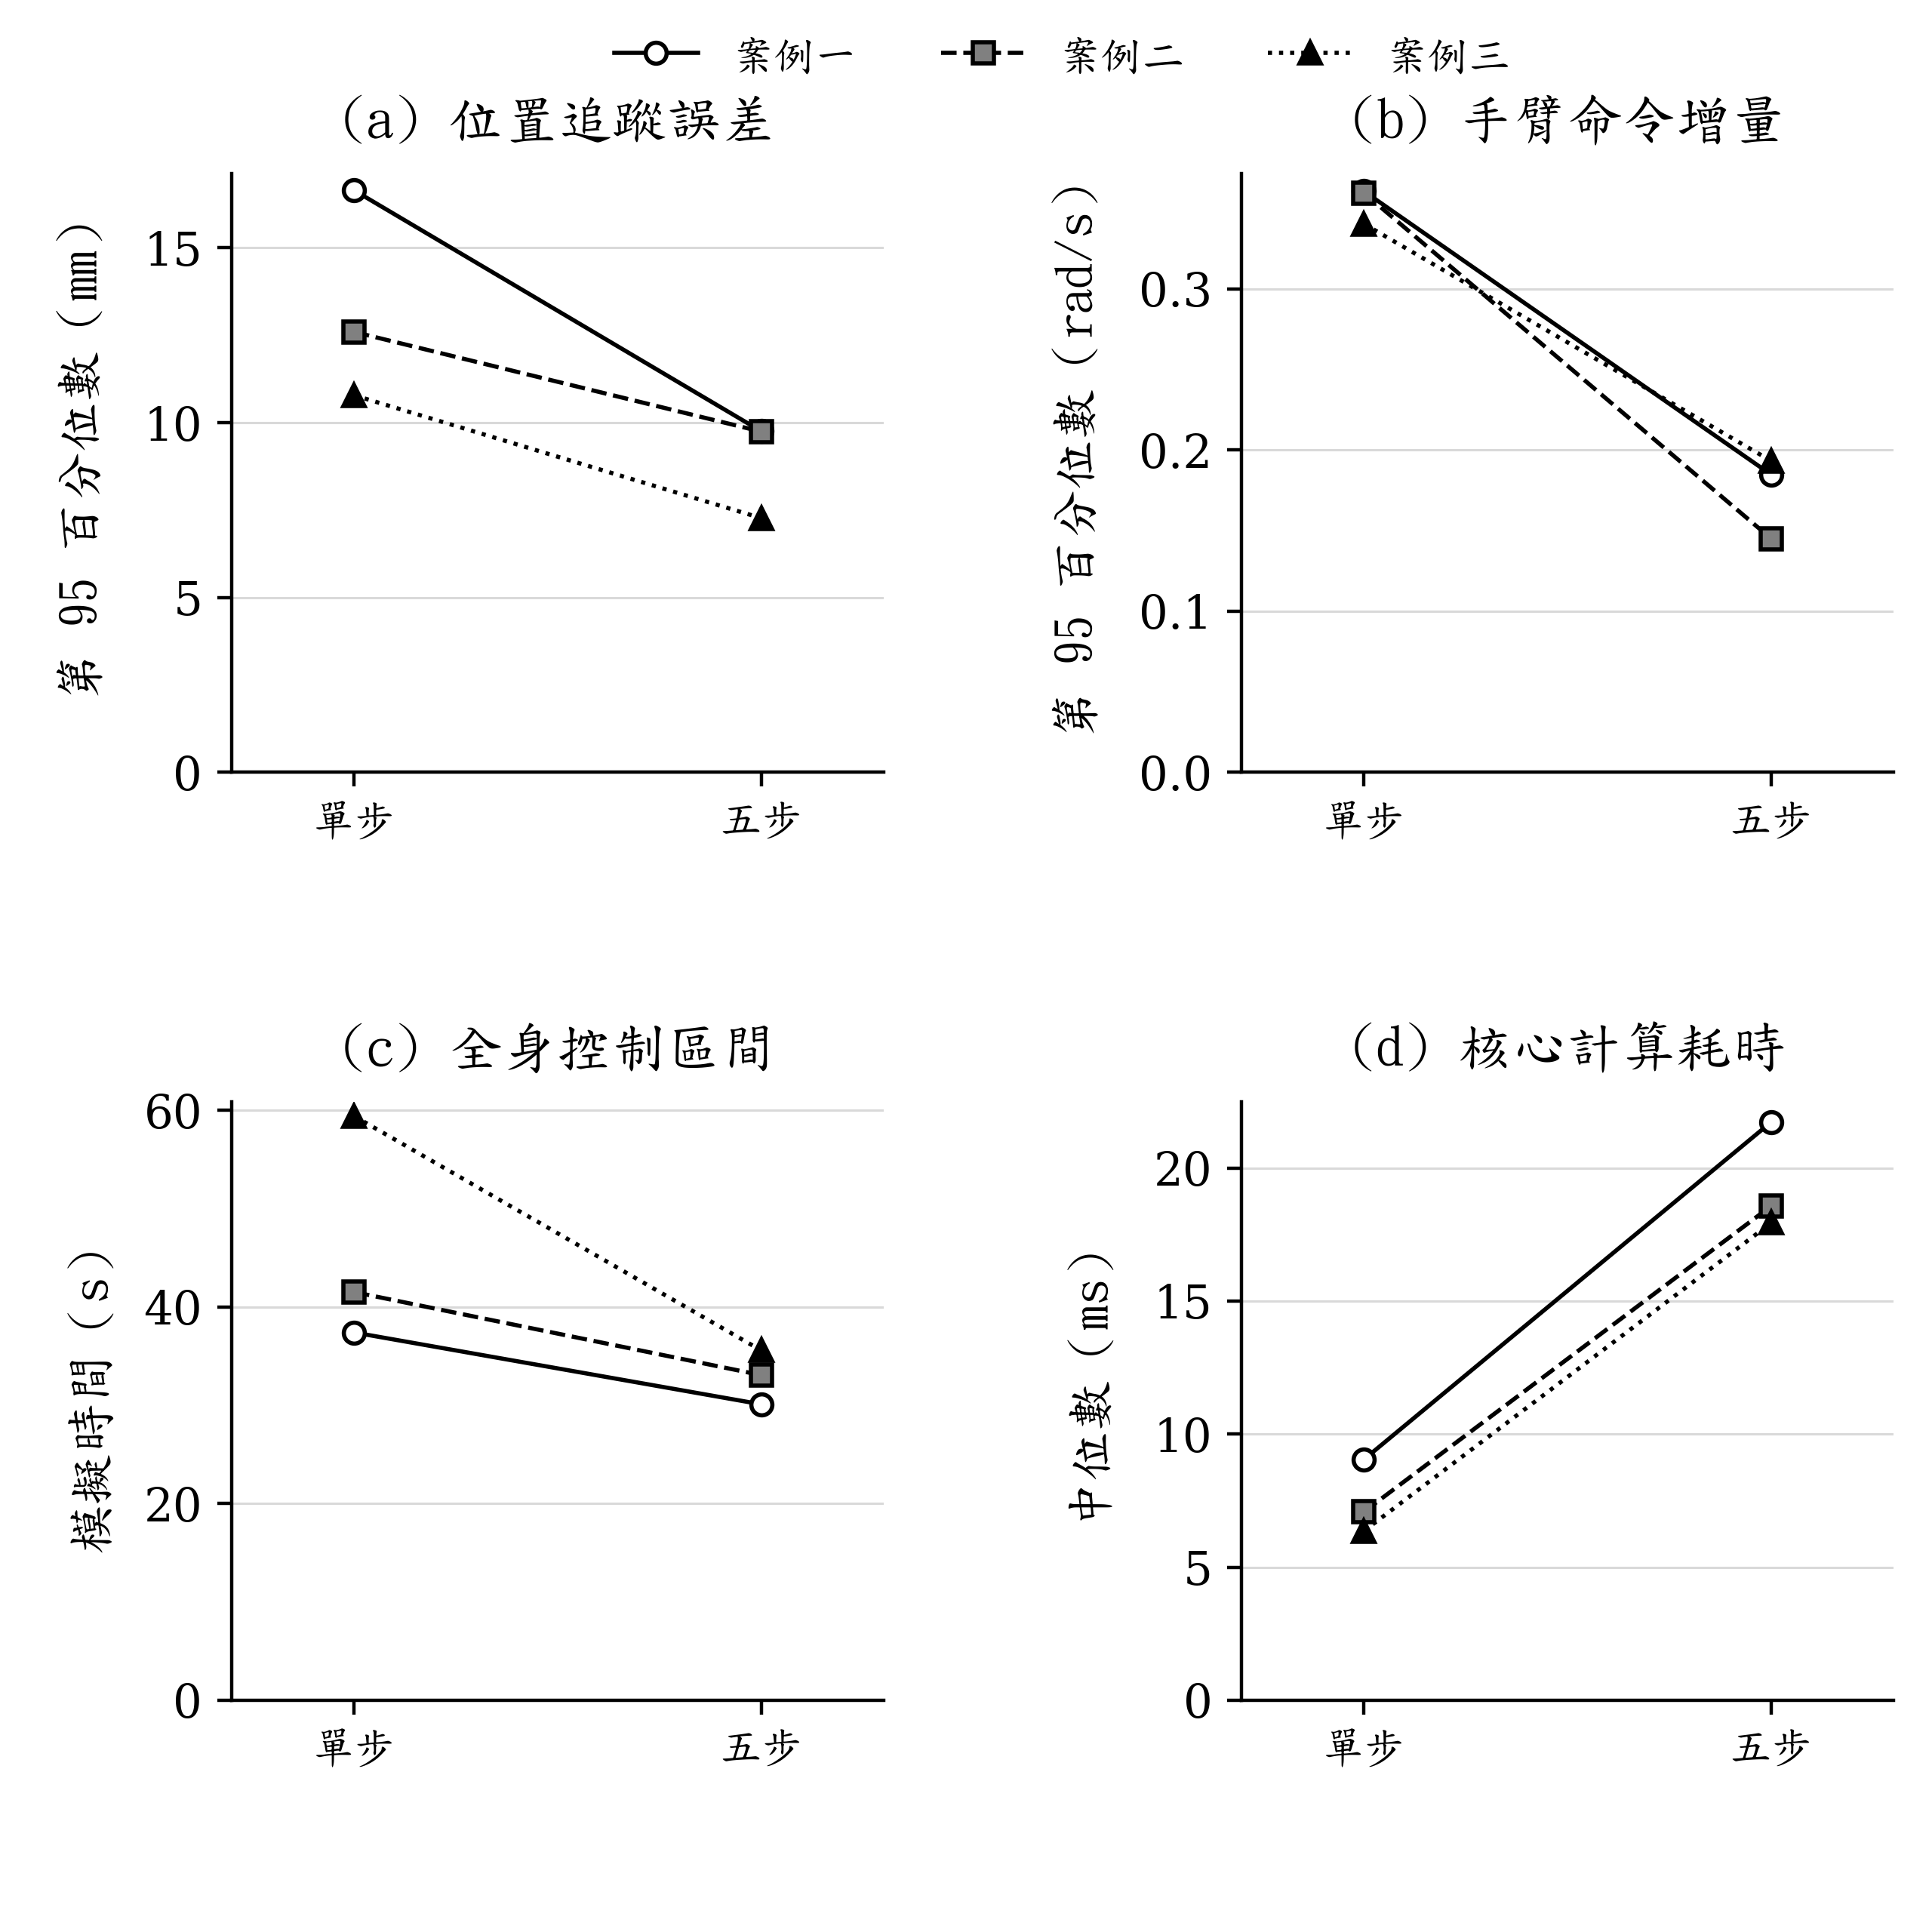
\includegraphics[width=0.98\textwidth]{figsrc/ch04/horizon_tracking_comparison.png}
    \caption{單步與五步控制之配對比較：
    (a) 位置誤差第 $95$ 百分位數；
    (b) 手臂命令增量第 $95$ 百分位數；
    (c) 全身控制區間；(d) 核心計算耗時中位數。
    各線連接同一配對案例；(c) 使用模擬時間，(d) 使用主機時間。}
    \label{fig:ch4_horizon_tracking_comparison}
\end{figure}

五步控制的控制區間分別為 $30.10$、$33.07$ 與 $35.58$ s，
相對應的單步配置則為 $37.41$、$41.52$ 與 $59.43$ s，
配對差介於 $7.31$--$23.85$ s。
五步配置的核心計算耗時中位數較高，
呈現單次計算成本與任務推進時間之間的取捨。
此處計算耗時包含當時求解流程的局部近似與最佳化運算，
各組的執行順序與主機熱狀態仍有差異，
其耗時差值須連同執行條件解讀。

整段統計的改善亦有階段差異。
例如配對案例二在開啟保持階段，
單步與五步的位置誤差第 $95$ 百分位數分別約為 $0.91$ 與 $1.47$ mm，
該階段由單步配置取得較低誤差。
本組三對資料據此支持五步配置在整段追蹤、命令變化與控制區間上的改善，
其適用範圍仍限於上述抽屜任務、成本與控制設定。

% ==================================================
% 4.4.3 抽屜操作之移動與停駐策略比較
% ==================================================
\subsection{抽屜操作之移動與停駐策略比較}
\label{subsec:moving_parked_drawer_strategy}

操作策略比較另採用三組配對資料，兩組皆使用五步全身控制。
移動中操作允許底盤在接近與開關抽屜期間配合手臂移動；
停駐後操作則先完成底盤減速與定位，再以位置保持伺服維持底盤，
由手臂完成接近、拉開與推回。
兩組共用抽屜、起終點、開關保持條件及當時的偏置觀測設定，
並交替安排執行順序。
停駐組另固定預測期間的底盤輸入並停用近目標命令整形，
因此本項比較涵蓋進場、接手與運動安排等完整策略的差異。

完整任務時間以模擬時鐘計算，
由首次發布導航計畫起算，至開啟與關閉保持條件皆完成、
控制權已交還導航，且底盤首次返回起點 $0.20$ m 範圍內為止。
任務完成時間由逐物理步狀態獨立判定，
並與任務結束事件交叉核對，兩者差異皆不超過 $0.04$ s。
此時間涵蓋進場、接近、開關、退出、收臂與返回，
與前節僅涵蓋全身控制的評估區間分別計算。

停駐條件亦在實際接手至交還導航的完整區間內核對。
三個停駐案例的最大底盤平移速度為 $0.930$--$0.975$ mm/s，
相對停駐錨點的最大位置偏差為 $0.479$--$0.487$ mm，
最大朝向偏差為 $0.207$--$0.250^\circ$，
皆符合所設定的 $1$ mm/s、$1$ mm 與 $0.5^\circ$ 上限。
此核對使停駐策略的結果能對應至實際底盤保持狀態。

\cref{tab:ch4_moving_parked_drawer_results}列出完整任務時間。
六個案例皆完成開關抽屜與返回，
移動策略的平均時間為 $80.72$ s，停駐策略為 $93.62$ s。
三組配對皆由移動策略取得較短時間，
縮短量為 $12.51$--$13.19$ s，
依式\eqref{eq:ch4_task_time_comparison}計算的時間縮短比例為 $13.38$--$14.05\%$。

\begin{table}[htbp]
    \centering
    \caption{移動中操作與停駐後操作之完整任務時間比較}
    \label{tab:ch4_moving_parked_drawer_results}
    \begingroup
    \small
    \setlength{\tabcolsep}{5pt}
    \renewcommand{\arraystretch}{1.25}
    \begin{tabular}{c c c c c}
        \hline
        配對案例
        & \shortstack{移動中操作\\（s）}
        & \shortstack{停駐後操作\\（s）}
        & \shortstack{時間縮短\\（s）}
        & \shortstack{縮短比例\\（\%）} \\
        \hline
        一 & $80.99$ & $93.50$ & $12.51$ & $13.38$ \\
        二 & $80.70$ & $93.89$ & $13.19$ & $14.05$ \\
        三 & $80.46$ & $93.48$ & $13.02$ & $13.93$ \\
        \hline
    \end{tabular}
    \endgroup
\end{table}

\cref{fig:ch4_moving_parked_drawer_comparison}(b)將時間差依任務事件分段。
由出發至全身接手的平均時間差約為 $11.40$ s，
包含進場減速、位置與朝向收斂及不同接手條件。
停駐組的靜止觀察區間約為 $0.51$ s，
僅占上述差距的一部分。
全身接手至夾持成立期間，移動策略平均多用約 $1.90$ s；
若改由共同出發事件計算至夾持成立，
移動策略仍較快 $9.09$--$9.76$ s。
因此，較早接手帶來的時間收益，
需與接手後仍持續進行的接近及穩定過程一併評估。

\begin{figure}[htbp]
    \centering
    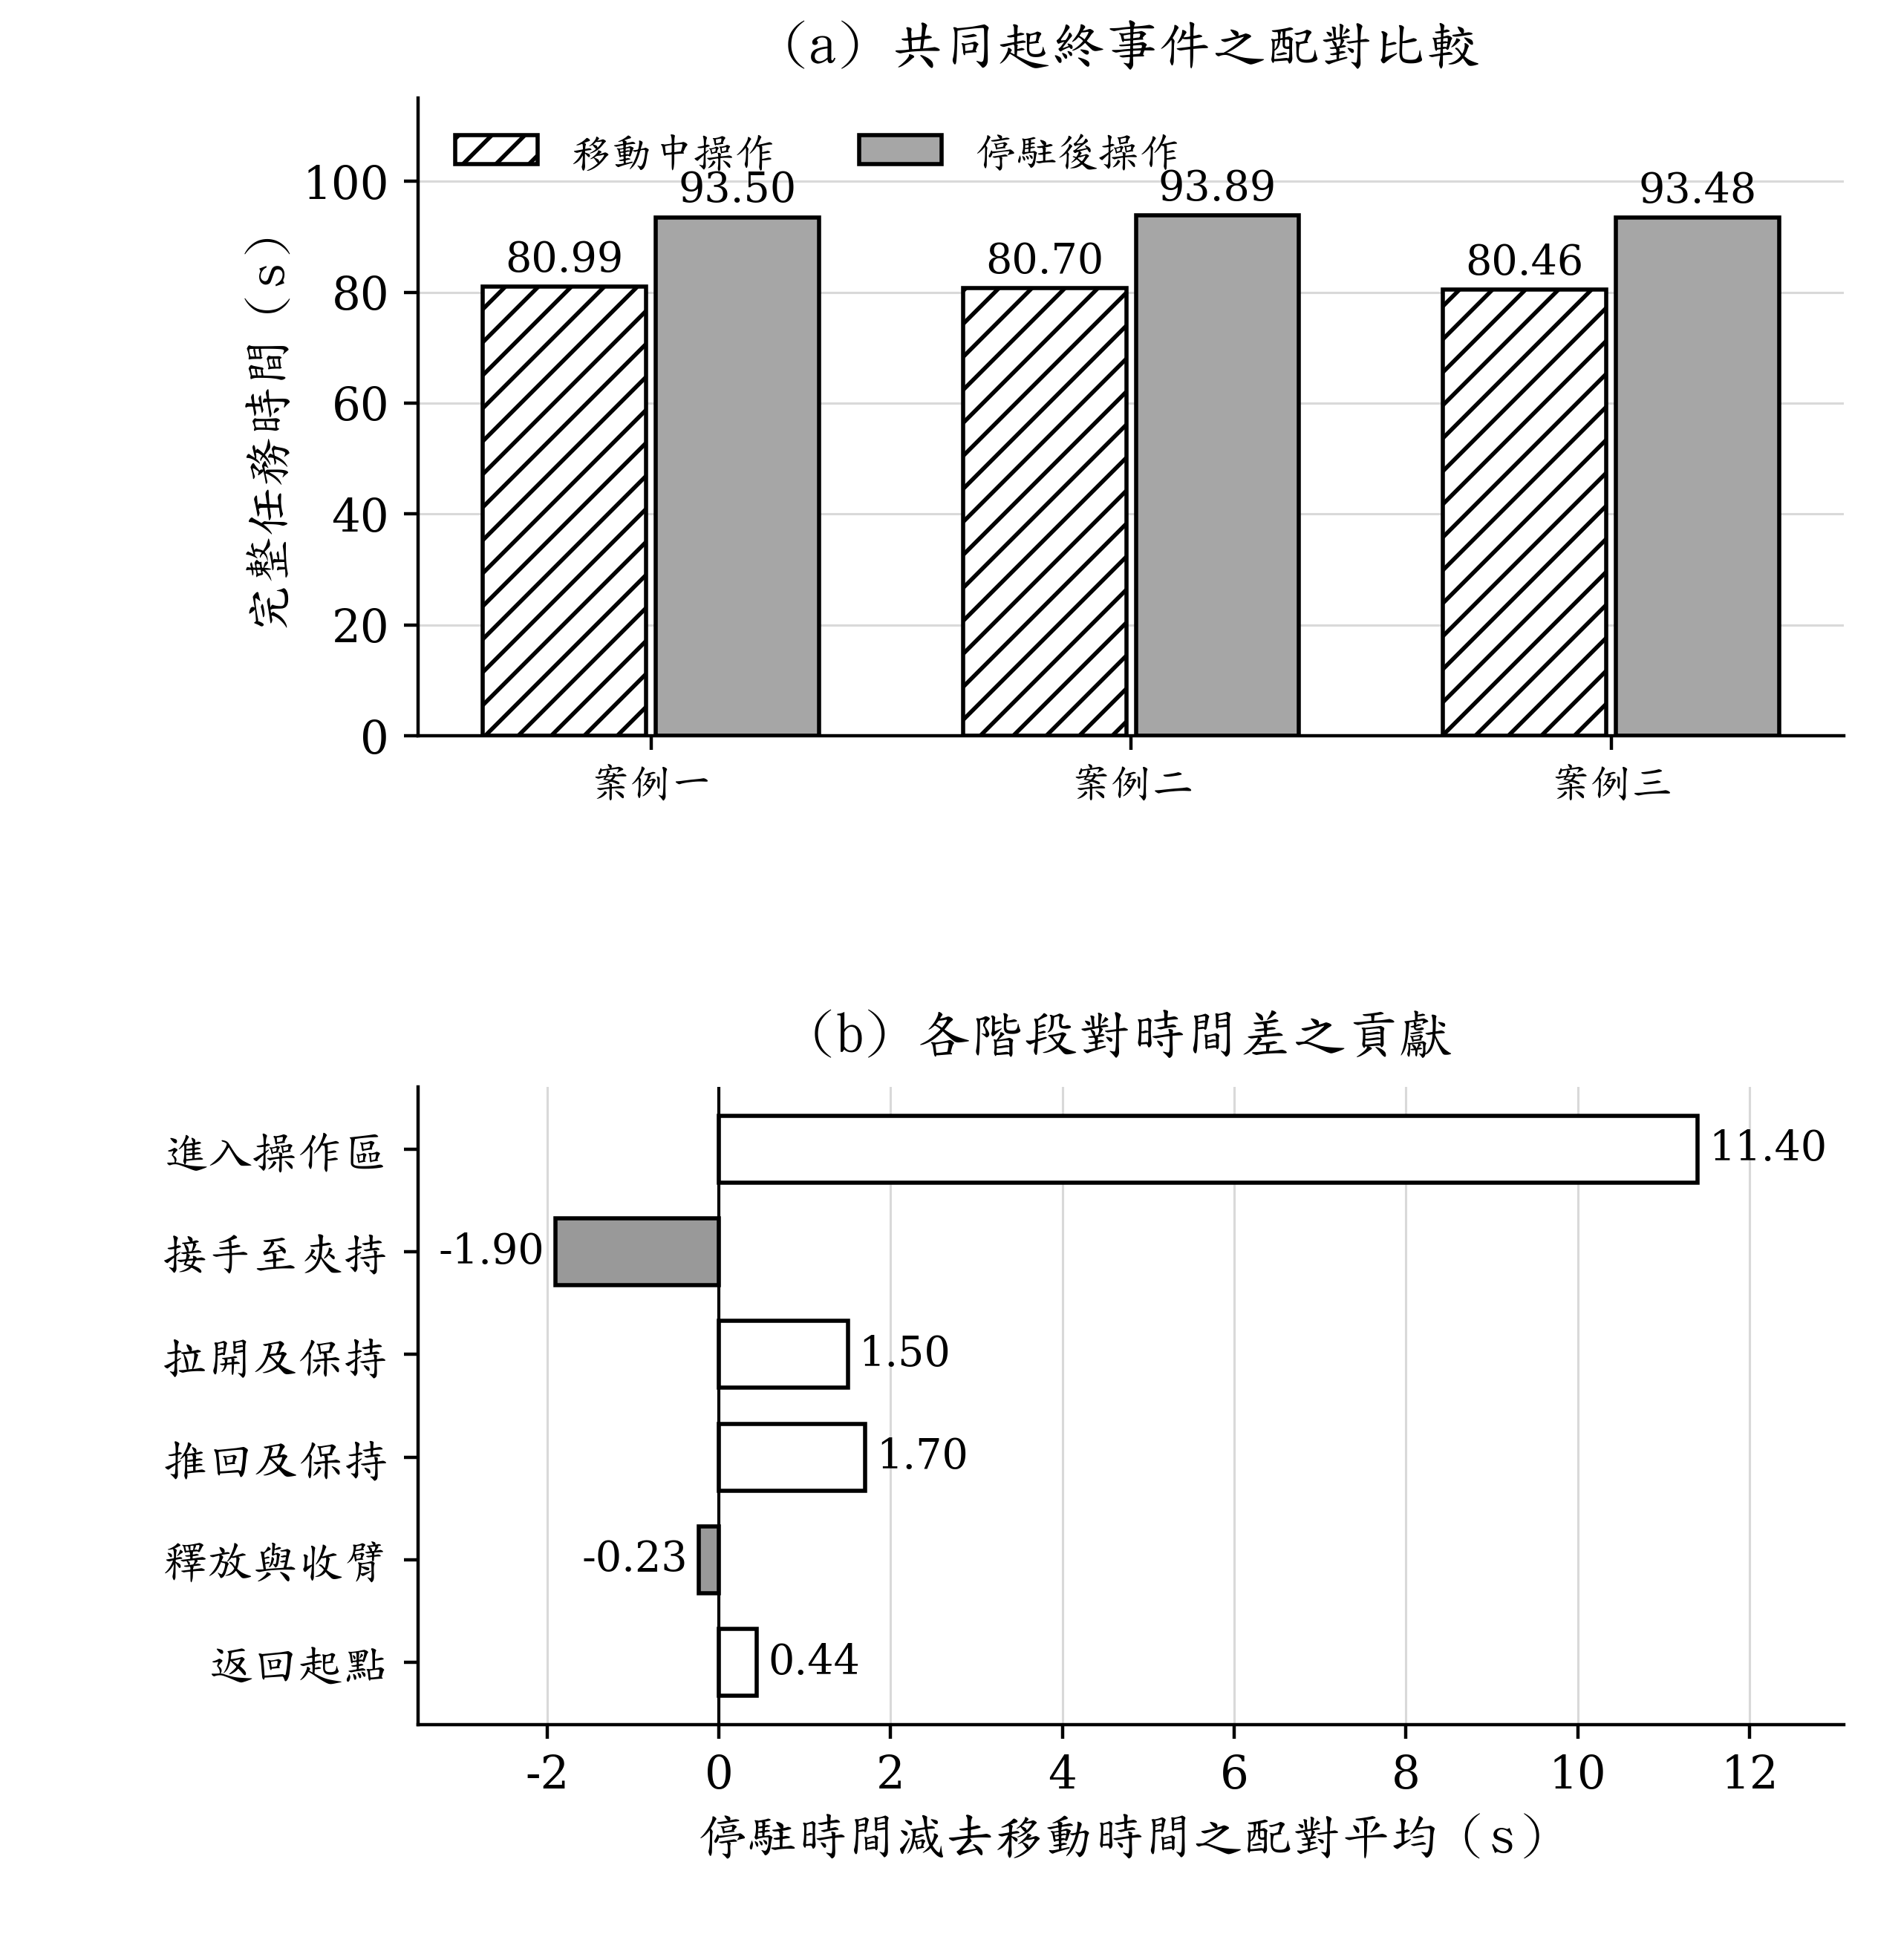
\includegraphics[width=0.98\textwidth]{figsrc/ch04/moving_parked_drawer_comparison.png}
    \caption{抽屜操作之策略比較：
    (a) 三組配對的完整任務時間；
    (b) 各階段之停駐時間減去移動時間的配對平均值。
    正值表示移動策略在該階段較省時，負值表示移動策略用時較長；
    各階段時間差之和對應完整任務的平均時間差。}
    \label{fig:ch4_moving_parked_drawer_comparison}
\end{figure}

拉開與開啟保持、推回與關閉保持兩段，
移動策略分別平均縮短約 $1.50$ 與 $1.70$ s；
釋放與收臂階段則平均增加約 $0.23$ s，
返回階段平均縮短約 $0.44$ s。
完整時間差主要來自進場與接手安排，
其次為開關抽屜期間的協同運動。

操作品質方面，六個案例在拉開階段的雙指接觸力皆持續達到 $0.5$ N，
但夾持期間最大相對位移的配對結果並未呈現相同方向。
移動策略的三個值為 $1.583$、$0.057$ 與 $0.251$ mm，
停駐策略則為 $0.092$、$0.095$ 與 $0.131$ mm，
兩組皆通過所設定的 $10$ mm 位移上限。
這些結果支持本組移動策略在完成既定操作條件下縮短完整任務時間，
夾持品質則須依其接觸與相對位移分別評估。
上述比較以三組配對案例描述本場景下的觀察，
後續住宅任務再檢查視覺目標、導航與多階段操作的整體銜接。
